%=====================
\chapter{Requirements}
%=====================
\label{chap:req:requirements}
This chapter describes an utility that creates Wireshark dissectors from C
header files. The dissectors must interpret binary representations of C
structs. In \autoref{sec:req:list} we give a high level overview of the
utility and lists all the functional and non-function requirements.

\hyperref[sec:req:stories]{Section \ref*{sec:req:stories}} gives user stories
for the requirements, while \autoref{sec:req:usecases} provides use cases for
the utility, and \autoref{sec:prodbacklog} contains the complete product
backlog.

%-----------------------------
\section{List of requirements}
%-----------------------------
\label{sec:req:list}

\subsection{Overview}
%-----------------
We are to create an utility that allows Wireshark to interpret the binary
representations of C-language structs. While C structs seldom are exchanged
across networks, they are sometimes used in inter-process communication. The
purpose of the utility described here is to provide Wireshark with the
capability of automatically dissecting the binary representation of a C struct,
as long as its definition is known.

The expected work flow for the utility is to read one or more C header files,
which contain struct definitions, and output Wireshark dissectors, implemented
in Lua scripts. A configuration file or source code annotations in the header
files may be used when additional configuration is required.

\autoref{tab:req:func} lists the functional requirements, while
\autoref{tab:req:nonfunc} lists the non-functional requirements. Each
requirement have a priority (Pri) and a complexity (Cmp): High (H), 
Medium (M) or Low (L) which is explained in \autoref{sec:req:priority} and
\autoref{sec:req:compl}.

\subsection{Prioritization}
%--------------------------
\label{sec:req:priority}
The team has, in cooperation with the customer, prioritized the requirements
in three categories:
\begin{inparaenum}[\itshape a\upshape)]
	\item High,
	\item Medium or
	\item Low.
\end{inparaenum} 

\begin{description}
	\item[High] Core functionality of the utility which must be implemented.
	\item[Medium] Requirements that will improve the value of the utility.
	\item[Low] Requirements that will not add much value to the utility.
\end{description}

\subsection{Complexity}
%----------------------
\label{sec:req:compl}
The team has estimated the complexity for each requirement. We use the same
categories as for requirements priority:
\begin{inparaenum}[\itshape a\upshape)]
	\item High,
	\item Medium or
	\item Low.
\end{inparaenum} 

\begin{description}
	\item[High] Functionality which seems difficult and non-trivial to create.
	\item[Medium] Functionality that seems time consuming but straight forward.
	\item[Low] Requirements that are trivial to implement.
\end{description}

\begin{table}[htbp] \footnotesize \center
\caption{Functional Requirements\label{tab:req:func}}
\noindent\makebox[\textwidth]{%
\begin{tabularx}{1.2\textwidth}{l X c c}
	\toprule
	ID & Description & Pri. & Cmp. \\
	\midrule
	FR1 & The utility must be able to read basic C language struct definitions from C header files & H & \\
	FR1-A & The utility must support the following basic data types: int, float, char and boolean & H & L \\
	FR1-B & The utility must support members of type enums & H & L \\
	FR1-C & The utility must support members of type structs & H & M \\
	FR1-D & The utility must support members of type unions & M & M \\
	FR1-E & The utility must support member of type array & H & M \\
	\midrule
	FR2 & The utility must be able to generate lua-script for Wireshark dissectors for the binary representation of C struct & H & \\
	FR2-A & The dissector shall be able to display simple structs & H & L \\
	FR2-B & The dissector shall be able to support structs within structs & M & M \\
	FR2-C & The dissector must support Wiresharks built-in filter and search on attributes & H & L \\
	FR2-D & The dissector shall be able to recognize invalid values for a struct member & L & L \\
	\midrule
	FR3 & The utility must support C preprocessor directives and macros & H & \\
	FR3-A & The utility shall support \#include & H & L \\
	FR3-B & The utility shall support \#define and \#if & H & L \\
	FR3-C & The utility shall support \verb+WIN32+, \verb+_WIN32+, \verb+_WIN64+, \verb+__sparc__+, \verb+__sparc+ and \verb+sun+ & M & H \\
	\midrule
	FR4 & The utility must support user configuration & M & \\
	FR4-A & Configuration must support valid ranges for struct members & L & L \\
	FR4-B & Configuration must support integer members which represent enumerated named value or a bit string & M & L \\
	FR4-C & Configuration must support custom handling of specific data types. E.g. a 'time\_t' may be interpreted to contain a unixtime value, and be displayed as a date & L & M \\
	FR4-D & Configuration must support specifying the ID of dissectors & - & - \\
	FR4-E & Configuration must support custom Lua files for specific protocols & - & - \\
	\midrule
	FR5 & A struct may have a header and/or trailer (other registered protocol). The configuration must support the use of integer members to indicate the number of other structs that will follow in the trailer & L & H \\
	\midrule
	FR6 & The dissectors must be able to handle binary input which size and endian depends on originating platform & M & \\
	FR6-A & Flags must be specified in configuration for each platform & M & M \\
	FR6-B & Flags within message headers should signal the platform & M & H \\
	FR6-C & Generate dissectors which support both little and big endian platforms & - & - \\
	FR6-D & Generate dissectors which support different sizes depending on platforms & - & - \\
	\midrule
	FR7 & The utility shall support parameters from command line & H & \\
	FR7-A & Command line shall support parameters for c-header file & H & L \\
	FR7-B & Command line shall support for configuration file & H & L \\
	FR7-C & Command line shall support batch mode of c-header and configuration file & L & M \\
	FR7-D & When running batch mode, dissectors that already are generated, shall not be regenerated, if the source are not modified since last run & L & M \\
	\bottomrule
\end{tabularx}}
\end{table}

\begin{table}[htbp] \footnotesize \center
\caption{Non-Functional Requirements\label{tab:req:nonfunc}}
\noindent\makebox[\textwidth]{%
\begin{tabularx}{1.2\textwidth}{l X c c}
	\toprule
	ID & Description & Pri. & Cmp. \\
	\midrule
	NR1 & The utility shall be able to run on latest Windows and Solaris operating system & M & L \\
	\addlinespace
	NR2 & The dissector shall be able to run on Windows x86, Windows x86-64, Solaris x86, Solaris x86-64 and Solaris SPARC & M & M \\
	\addlinespace
	NR3 & The utilities user interface shall be command line. No clicking! & H & L \\
	\addlinespace
	NR4 & The configuration shall have sufficient documentation to allow a person with no previous knowledge of the system to be able to use it to generate LUA-scripts after X hours of reading & M & M \\
	\addlinespace
	NR5 & The configuration should have sufficient documentation to allow a person, already proficient with the system, to understand the code well enough to be able to extend it’s functionality after Y hours of reading & M & M \\
	\addlinespace
	NR6 & The utility code should follow standard python coding convention as specified by PEP8, and try to follow python style guidelines defined by PEP20 & H & L \\
	\addlinespace
	NR7 & The utilities code should be documented by python docstrings which should explain the use of the code. Python modules, classes, functions and methods should have docstrings & M & L \\
	\bottomrule
\end{tabularx}}
\end{table}


%---------------------
\section{User Stories}
%---------------------
\label{sec:req:stories}
This sections shows the user stories, these are display in
\autoref{tab:req:stories1} and \autoref{tab:req:stories2}. The developer in
this context is the developers at Thales Norway AS. The administrator is this
context is the users of the dissectors.

\begin{table}[htbp] \footnotesize \center
\caption{User stories part 1\label{tab:req:stories1}}
\noindent\makebox[\textwidth]{%
\begin{tabularx}{1.2\textwidth}{l X}
	\toprule
	Header. & Value \\
	\midrule
	ID:			& US01 \\
	Requirements:	& FR01A, FR03B, FR07A \\
	User Story:		& As a developer I want to generate a Lua-script from command-line from a C header file with a struct using basic C data types, so I get a dissector for Wireshark \\
	\midrule
	ID:			& US02 \\
	Requirements:	& FR02A \\
	User Story:		& As an administrator,, I want to use the dissector for simple structs in Wireshark, so that I can display structs without binary representation. \\
	\midrule
	ID:			& US03 \\
	Requirements:	& FR04A, FR07B \\
	User Story:		& As a developer, I want to configure allowed ranges for struct members, so that I can display invalid values in the dissector. \\
	\midrule
	ID:			& US04 \\
	Requirements:	& FR02D \\
	User Story:		& As an administrator, I want to see invalid struct values in wireshark, so that I easier can easier can recognize invalid values. \\
	\midrule
	ID:			& US05 \\
	Requirements:	&  FR01C, FR03A \\
	User Story:		& As a developer, I want to support structs with structs, so that I can generate dissector for Wireshark \\
	\midrule
	ID:			& US06 \\
	Requirements:	& FR02B \\
	User Story:		&  As an administrator, I want to use the dissector for structs with other structs in Wireshark, so that I can display structs without binary representation. \\
	\midrule
	ID:			& US07 \\
	Requirements:	&  FR02C \\
	User Story:		&  As an administrator, I want to use Wireshark built-in filter and search, so that I easier can find attributes. \\
	\bottomrule
\end{tabularx}}
\end{table}

\begin{table}[htbp] \footnotesize \center
\caption{User stories part 2\label{tab:req:stories2}}
\noindent\makebox[\textwidth]{%
\begin{tabularx}{1.2\textwidth}{l X}
	\toprule
	Header. & Value \\
	\midrule
	ID:			& US08 \\
	Requirements:	&  FR01B, FR03B, FR04B \\
	User Story:		& As a developer, I want support for integer member which represent enumerated value or bit string in the configuration, so that I can display named values in the dissector. \\
	\midrule
	ID:			& US09 \\
	Requirements:	& FR01D, FR01E \\
	User Story:		& As a developer, I want to support structs wither unions and arrays, so that I can generate Lua-scripts for more complex C structs. \\
	\midrule
	ID:			& US10 \\
	Requirements:	&  FR07C, FR07D \\
	User Story:		& As a developer, I want to generate Lua-script in batch mode, without regenerating header files that are not modified since last, so that I can generate several Lua-scripts faster. \\
	\midrule
	ID:			& US11 \\
	Requirements:	&  FR05 \\
	User Story:		& As a developer, I want support in configuration to handle structs with header and/or trailer, so that I can display structs sent in a serie. \\
	\midrule
	ID:			& US12 \\
	Requirements:	&  FR03B, FR03C \\
	User Story:		& As a developer I want support for C preprocessor directives and macro, so that I am able to generate Lua-scripts from c header files that are created for use on multiple platforms. \\
	\midrule
	ID:			& US13 \\
	Requirements:	& FR06A, FR06B \\
	User Story:		& As a developer, I want dissectors that are able to handle binary input which size and endian depends on originating platform, so that I can display these values correctly in Wireshark.  \\
	\bottomrule
\end{tabularx}}
\end{table}


%------------------
\section{Use Cases}
%------------------
\label{sec:req:usecases}
This sections contains use case diagrams for our two actors, and detailed
textual use cases for these diagrams.

\subsection{Actors}
%------------------
An actor specifies a role played by an external person or thing that interact
with our utility. We have three types of actors to consider. First is the
primary actor which in our case is the user of our utility. He who feeds it a
C file to generate dissectors. A secondary actor is someone who configures our
utility to change the output of it. Finally we have an offstage actor which
does not use our utility himself, but uses the output dissectors in Wireshark.

We have defined two use case actors for our utility. The customer has specified
that the offstage actor, called administrator, is the most important actor.
\begin{description}
	\item[Administrator] User of the generated Wireshark dissectors, offstage actor
	\item[Developer] User and configurer of utility, primary and secondary actor
\end{description}

\subsection{Use Case Diagrams}
%-----------------------------
\hyperref[fig:req:ucadm]{Figure \ref*{fig:req:ucadm}} shows the use case
diagram for the administrator, and \autoref{fig:req:ucdev} is the use case
diagram for the developer.x
\begin{figure}[htbp]
	\center
	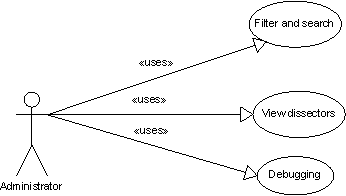
\includegraphics[width=0.8\textwidth]{./planning/img/administrator.png}
	\caption{Use Case Diagram: Administrator\label{fig:req:ucadm}}
\end{figure}

\begin{figure}[htbp]
	\center
	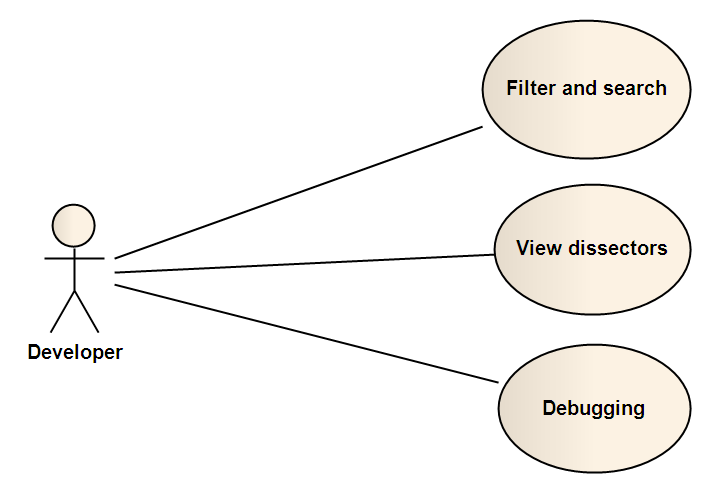
\includegraphics[width=0.8\textwidth]{./planning/img/developer.png}
	\caption{Use Case Diagram: Developer\label{fig:req:ucdev}}
\end{figure}

\subsection{Textual Use Cases}
%-----------------------------
TODO!!!

